% Build (from docs/tex):  xelatex -interaction=nonstopmode solution.tex  (run twice for the table of contents)
\documentclass[10.5pt,a4paper]{article}
\usepackage[a4paper,top=2.2cm,bottom=2.2cm,left=2.1cm,right=2.1cm,headheight=14pt]{geometry}
\usepackage{fontspec}
\setmainfont{Segoe UI}
\setsansfont{Segoe UI}
\setmonofont{Consolas}[Scale=0.92]
\newfontfamily\headfont{Segoe UI Semibold}
\usepackage{xeCJK}
\setCJKmainfont{Microsoft YaHei}
\setCJKmonofont{Microsoft YaHei}
\xeCJKDeclareCharClass{Default}{"00B7,"2013,"2014,"2018,"2019,"201C,"201D,"2026,"2192,"2264,"2265,"03A3}
\usepackage[table]{xcolor}
\usepackage{graphicx,tabularx,booktabs,array,enumitem,fancyhdr,titlesec,amsmath}
\usepackage[most]{tcolorbox}
\usepackage{fvextra}
\usepackage[hidelinks]{hyperref}

% ---------------------------------------------------------------- palette
\definecolor{brand}{HTML}{1A73E8}
\definecolor{brandsoft}{HTML}{E8F0FE}
\definecolor{ink}{HTML}{202124}
\definecolor{mute}{HTML}{5F6368}
\definecolor{line}{HTML}{DADCE0}
\definecolor{rowalt}{HTML}{F6F8FB}
\definecolor{green}{HTML}{188038}
\definecolor{greensoft}{HTML}{E6F4EA}
\definecolor{amber}{HTML}{E37400}
\definecolor{ambersoft}{HTML}{FEF7E0}
\definecolor{codebg}{HTML}{F8F9FA}
\color{ink}

% ---------------------------------------------------------------- layout
\setlength{\parindent}{0pt}
\setlength{\parskip}{5pt}
\linespread{1.12}
\setlist{itemsep=2pt,topsep=3pt,leftmargin=1.4em}
\setlist[itemize]{label={\color{brand}\textbullet}}
\renewcommand{\arraystretch}{1.35}
\titleformat{\section}{\headfont\LARGE\color{brand}}{\thesection}{0.6em}{}[\vspace{-4pt}{\color{line}\titlerule[1pt]}]
\titleformat{\subsection}{\headfont\Large\color{ink}}{\thesubsection}{0.6em}{}
\titleformat{\subsubsection}{\headfont\large\color{brand}}{\thesubsubsection}{0.6em}{}
\titlespacing*{\section}{0pt}{18pt}{10pt}
\titlespacing*{\subsection}{0pt}{14pt}{6pt}
\titlespacing*{\subsubsection}{0pt}{12pt}{4pt}
\pagestyle{fancy}\fancyhf{}
\fancyhead[L]{\small\color{mute}R2AI 2026 · Stage 3 · Đội chande}
\fancyhead[R]{\small\color{mute}Tài liệu thuyết minh sản phẩm}
\fancyfoot[C]{\small\color{mute}\thepage}
\renewcommand{\headrulewidth}{0.4pt}
\renewcommand{\headrule}{{\color{line}\hrule height\headrulewidth}}
\fvset{breaklines,breakanywhere,fontsize=\small}

% ---------------------------------------------------------------- boxes
\newtcolorbox{note}[1][]{enhanced,breakable,colback=brandsoft,colframe=brandsoft,borderline west={3pt}{0pt}{brand},
  arc=2pt,left=10pt,right=8pt,top=6pt,bottom=6pt,#1}
\newtcolorbox{codebox}[1]{enhanced,breakable,colback=codebg,colframe=line,boxrule=0.5pt,arc=3pt,
  left=8pt,right=8pt,top=4pt,bottom=4pt,title={\small\headfont #1},coltitle=mute,colbacktitle=codebg,
  attach boxed title to top left={yshift=-2.2mm,xshift=4mm},boxed title style={colframe=line,boxrule=0.5pt,arc=2pt}}
\newtcolorbox{card}[2]{enhanced,colback=white,colframe=#1,boxrule=0.8pt,arc=4pt,
  title={\headfont #2},colbacktitle=#1,coltitle=white,left=8pt,right=8pt,top=4pt,bottom=6pt,equal height group=cards}
\newcommand{\metric}[2]{\begin{tcolorbox}[enhanced,colback=white,colframe=line,boxrule=0.6pt,arc=4pt,width=\linewidth,
  halign=center,top=6pt,bottom=6pt]{\headfont\fontsize{20}{22}\selectfont\color{brand}#1}\\[2pt]{\small\color{mute}#2}\end{tcolorbox}}
\newcolumntype{Y}{>{\raggedright\arraybackslash}X}
\newcommand{\thead}[1]{\leavevmode\textbf{#1}}
\newenvironment{nicetable}[1]{\rowcolors{2}{rowalt}{white}\tabularx{\linewidth}{#1}\toprule}{\endtabularx}
\newcommand{\code}[1]{\colorbox{brandsoft}{\small\texttt{#1}}}

\begin{document}

% ================================================================= cover
\thispagestyle{empty}
\begin{tcolorbox}[enhanced,colback=brand,colframe=brand,arc=0pt,left=18pt,right=18pt,top=22pt,bottom=22pt,
  width=\paperwidth,enlarge left by=-2.1cm,enlarge top by=-2.2cm,spread sidewards=0pt]
\color{white}
{\small R2AI 2026 · STAGE 3 · TÀI LIỆU THUYẾT MINH SẢN PHẨM}\\[10pt]
{\headfont\fontsize{26}{31}\selectfont Truy hồi tài liệu y khoa đa ngữ}\\[6pt]
{\large bge-m3 hybrid · mở rộng truy vấn đa ngữ · weighted Reciprocal Rank Fusion}
\end{tcolorbox}

\vspace{14pt}
\begin{tabular}{@{}p{3.2cm}l@{}}
\thead{Đội} & {\bfseries\large chande} \quad {\color{mute}(tài khoản leaderboard: \texttt{chande})} \\
\thead{Thành viên} & Đàm Quang Đức \quad·\quad Vũ Hữu An \quad·\quad Nguyễn Trần Nghĩa \\
\thead{Mã nguồn} & \href{https://github.com/quaqducc/r2ai-stage3-medical-retrieval}{\color{brand}github.com/quaqducc/r2ai-stage3-medical-retrieval} \\
\thead{Ngày} & 04/11/2026 \\
\end{tabular}

\vspace{10pt}
\noindent\begin{minipage}[t]{0.235\linewidth}\metric{0,3577}{FINAL (vòng public)}\end{minipage}\hfill
\begin{minipage}[t]{0.235\linewidth}\metric{0,3900}{Docs F2}\end{minipage}\hfill
\begin{minipage}[t]{0.235\linewidth}\metric{0,3255}{Chunks F2}\end{minipage}\hfill
\begin{minipage}[t]{0.235\linewidth}\metric{7 / 50}{Thứ hạng}\end{minipage}

\vspace{8pt}
\begin{note}
\textbf{Tóm tắt.} Hệ thống trả lời 1.200 câu hỏi sức khoẻ tiếng Việt bằng cách tìm trong kho 1,22 triệu trang y khoa Việt – Trung – Anh. Chỉ một mô hình nhúng mở (\textbf{BGE-M3}) đảm nhận cả truy hồi ngữ nghĩa lẫn truy hồi từ khoá. Mỗi câu hỏi được \emph{hỏi theo nhiều cách}: câu gốc, bản dịch tiếng Trung do \textbf{Qwen3.5-9B} sinh ra, câu hỏi mở rộng bằng phản hồi giả (Rocchio), và truy hồi thẳng ở cấp tài liệu. Kết quả của 14 cách hỏi được gộp bằng RRF có trọng số. Hệ thống không huấn luyện mô hình nào, chạy offline trên CPU, và chỉ cần GPU cho bước nhúng corpus.
\end{note}

\vspace{4pt}
\renewcommand{\contentsname}{Mục lục}
\begingroup\titlespacing*{\section}{0pt}{6pt}{6pt}\tableofcontents\endgroup
\newpage

% ================================================================= 1
\section{Đội thi}

Đội \textbf{chande} gồm ba thành viên: \textbf{Đàm Quang Đức}, \textbf{Vũ Hữu An} và \textbf{Nguyễn Trần Nghĩa}. Công việc chia theo ba mảng của pipeline:

\begin{itemize}
  \item \textbf{Thu thập dữ liệu:} crawl 1,22 triệu URL trên 94 domain bằng nhiều nguồn dự phòng.
  \item \textbf{Xử lý dữ liệu:} trích nội dung sạch, phân đoạn nguyên văn và dựng chỉ mục.
  \item \textbf{Truy hồi:} xây pipeline truy hồi; kiểm chứng từng thay đổi bằng các lần nộp vòng public.
\end{itemize}

Bài nộp được báo cáo là \code{i\_dprf15}. Bốn bài còn lại ở vòng private (\texttt{j\_hh125}, \texttt{i\_dprf1}, \texttt{d12\_both075}, \texttt{i\_dprf05}) là các biến thể trọng số của cùng một pipeline.

% ================================================================= 2
\section{Mô hình sử dụng}

Hệ thống dùng đúng \textbf{hai mô hình mã nguồn mở}. Cả hai đều $\le$ 15B tham số, phát hành trước 01/08/2026 và được dùng nguyên checkpoint chính thức: \textbf{không fine-tune, không gọi API mô hình đóng}.

\vspace{4pt}
\noindent\begin{minipage}[t]{0.49\linewidth}
\begin{card}{brand}{BGE-M3 · 568M · nhúng văn bản}
\small
\textbf{Vai trò:} nhúng chunk và câu hỏi. Một lần chạy cho ra cả vector \textbf{dense} 1.024 chiều (ngữ nghĩa, xuyên ngôn ngữ) lẫn trọng số \textbf{sparse} (từ khoá).\par
\textbf{Checkpoint:} \href{https://huggingface.co/BAAI/bge-m3}{\color{brand}\texttt{BAAI/bge-m3}}\par
\textbf{Cấu hình:} FlagEmbedding 1.4.2, fp16. Corpus: tối đa 2.048 token, batch 32, GPU T4. Câu hỏi: tối đa 512 token, CPU.
\end{card}
\end{minipage}\hfill
\begin{minipage}[t]{0.49\linewidth}
\begin{card}{amber}{Qwen3.5-9B · 9B · dịch truy vấn}
\small
\textbf{Vai trò:} dịch câu hỏi tiếng Việt thành câu hỏi tiếng Trung (\texttt{zh\_q}) theo phong cách diễn đàn hỏi đáp, để khớp phần corpus tiếng Trung.\par
\textbf{Checkpoint:} \href{https://huggingface.co/unsloth/Qwen3.5-9B-GGUF}{\color{brand}\texttt{unsloth/Qwen3.5-9B-GGUF}}, file \texttt{Q4\_K\_M} (lượng tử hoá từ \texttt{Qwen/Qwen3.5-9B}).\par
\textbf{Cấu hình:} llama.cpp server, ngữ cảnh 16.384, 4 slot, \texttt{temperature=0}, \texttt{max\_tokens=1200}, tắt chế độ suy luận.
\end{card}
\end{minipage}

\vspace{6pt}
\begin{codebox}{Prompt của Qwen3.5-9B · 4-retrieve/retrieve/plan.py}
\begin{Verbatim}[fontsize=\footnotesize]
[system]
Bạn là chuyên gia y khoa song ngữ Việt–Trung–Anh, chuẩn bị truy vấn tìm kiếm cho một kho tài liệu y khoa gồm
bài báo/hỏi đáp tiếng Việt, diễn đàn hỏi đáp và bách khoa tiếng Trung, và tóm tắt PubMed tiếng Anh.
Chỉ trả về MỘT object JSON, không giải thích.

[user]
Câu hỏi của người bệnh (tiếng Việt):
{q}

Trả về JSON đúng các khoá sau:
{"type": "<một trong: symptom, disease, drug, pregnancy, pediatric, lab_result, nutrition, mental, procedure, other>",
 "vi_kw": "<từ khoá y khoa tiếng Việt, bỏ phần kể lể, giữ chỉ số/tên thuốc>",
 "zh_q": "<câu hỏi bằng tiếng Trung giản thể, viết như tiêu đề diễn đàn hỏi đáp y khoa (120ask, 39问医生)>",
 "zh_kw": "<thuật ngữ y khoa tiếng Trung, cách nhau bằng dấu cách>",
 "en_kw": "<medical English keywords, space separated, no AND/OR/quotes/brackets>",
 "entities": [{"vi": "<tên trong câu hỏi>", "en": "<tên chuẩn/hoạt chất>", "zh": "<tên tiếng Trung>"}],
 "subqs": [<chỉ khi câu hỏi có nhiều ý: mỗi ý là một câu hỏi tiếng Việt ngắn; ngược lại để []>]}
\end{Verbatim}
\end{codebox}

1.186/1.200 câu trả về JSON hợp lệ; câu lỗi thì chỉ dùng câu gốc. Bài nộp cuối chỉ dùng trường \texttt{zh\_q}.

% ================================================================= 3
\section{Tổng quan hệ thống}

\subsection{Bối cảnh và mục đích cuộc thi}

Người bệnh thường đặt câu hỏi sức khoẻ bằng ngôn ngữ đời thường. Còn tri thức trả lời được những câu hỏi ấy thì nằm rải rác trong báo chí, diễn đàn hỏi đáp và bách khoa tiếng Việt, tiếng Trung, cùng các bài tóm tắt PubMed tiếng Anh. Stage 3 của R2AI 2026 yêu cầu: với mỗi câu trong 1.200 câu hỏi tiếng Việt, tìm các tài liệu liên quan trong kho 1,22 triệu URL, kèm \textbf{đoạn trích nguyên văn} làm bằng chứng. Điểm là trung bình F2 cấp tài liệu và F2 cấp đoạn trích. F2 coi recall nặng gấp bốn lần precision, nên bài toán thưởng việc \emph{tìm đủ} hơn việc chỉ \emph{tìm đúng}.

\subsection{Tổng quan phương pháp và công nghệ}

\begin{note}
\textbf{Ý tưởng chính.} Thay vì thêm nhiều mô hình, chúng tôi dùng triệt để \emph{một} mô hình nhúng đa ngữ mạnh và tăng độ phủ bằng cách \textbf{hỏi cùng một câu theo nhiều cách}:
\begin{itemize}
  \item hỏi bằng câu gốc và bằng bản dịch tiếng Trung;
  \item hỏi bằng câu hỏi đã được "làm giàu" từ chính các kết quả đầu (Rocchio PRF);
  \item hỏi ở cấp đoạn và hỏi thẳng ở cấp tài liệu.
\end{itemize}
Mỗi cách hỏi cho một danh sách xếp hạng. RRF có trọng số gộp chúng thành một bảng xếp hạng duy nhất.
\end{note}

Hệ thống gồm hai pha. \textbf{Ingest} dựng kho văn bản và chỉ mục, chạy một lần. \textbf{Retrieve} trả lời 1.200 câu hỏi và chỉ mất vài phút khi đã có chỉ mục.

\begin{nicetable}{@{}p{3.6cm}Y@{}}
\thead{Lớp} & \thead{Công nghệ} \\ \midrule
Thu thập & Python, scrapling, trình duyệt headless cho site chống bot, Internet Archive Wayback, NCBI E-utilities (PubMed); lưu SQLite + zstd \\
Trích và làm sạch & trafilatura 2.0, lxml 5.3, luật XPath theo host, pyarrow / parquet \\
Mô hình & BGE-M3 qua FlagEmbedding 1.4.2 (PyTorch 2.6); Qwen3.5-9B GGUF qua llama.cpp \\
Chỉ mục và tìm kiếm & NumPy (ma trận dense float16, tìm chính xác bằng nhân ma trận), SciPy (ma trận sparse CSC), mmap. Không dùng vector database \\
Hạ tầng & Docker (3 image: extract, ingest, retrieve), Google Cloud Storage, VM GCP 16 vCPU, Google Colab T4 \\
\bottomrule
\end{nicetable}

\newpage
\subsection{Phương pháp chính}

\subsubsection{Ingest: từ danh sách URL đến chỉ mục}

\begin{center}
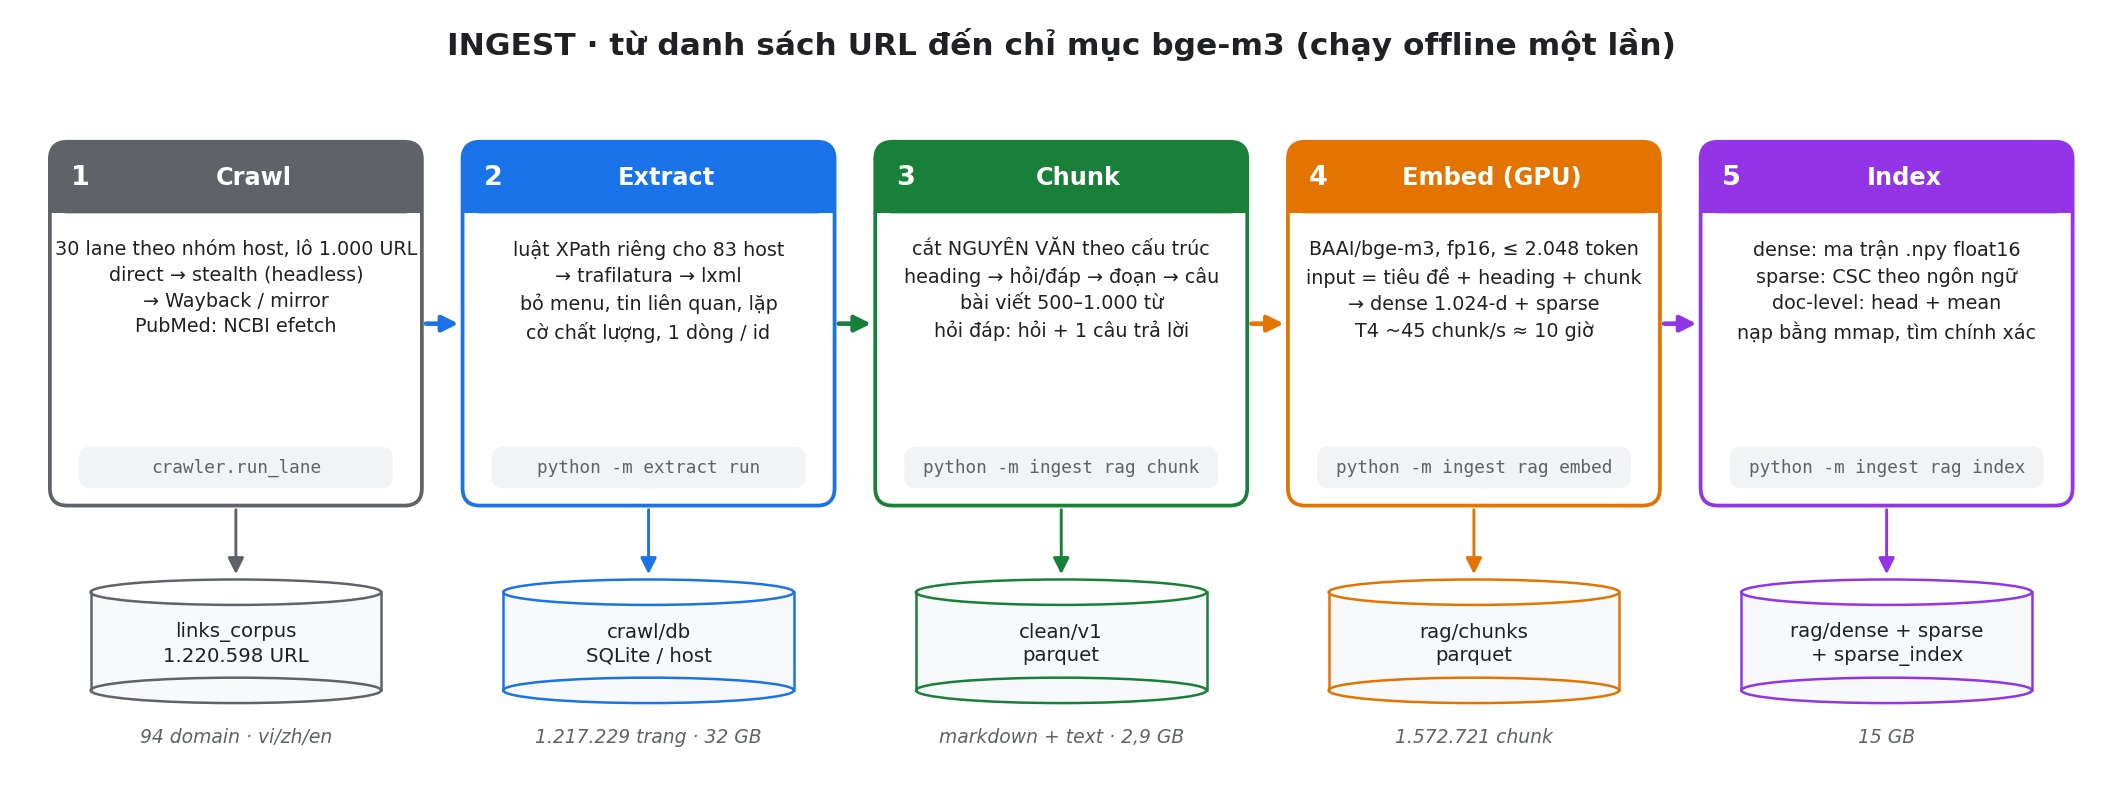
\includegraphics[width=\linewidth]{../img/ingest.png}\\[2pt]
{\small\color{mute}Hình 1. Pha ingest: năm bước, mỗi bước ghi ra một kho dữ liệu trung gian.}
\end{center}

\begin{enumerate}[label={\color{brand}\headfont\arabic*.},leftmargin=1.6em,itemsep=5pt]
\item \textbf{Crawl.} 1.220.598 URL được chia thành 30 lane theo nhóm host. Mỗi URL được thử lần lượt qua nhiều nguồn cho tới khi lấy được nội dung:

\begin{nicetable}{@{}p{4.2cm}>{\raggedleft\arraybackslash}p{2.2cm}Y@{}}
\thead{Nguồn} & \thead{Số trang} & \thead{Khi nào dùng} \\ \midrule
Tải trực tiếp & 889.782 & mặc định \\
NCBI efetch & 239.896 & toàn bộ PubMed (XML theo PMID) \\
Internet Archive & 73.193 & site gốc đã gỡ trang hoặc chặn \\
Trình duyệt headless & 9.069 & site chống bot \\
Mirror & 5.286 & site có bản mirror chính thức \\
\bottomrule
\end{nicetable}

Kết quả: \textbf{1.217.229 trang (99,72\%)}, mỗi host lưu trong một SQLite.

\item \textbf{Extract.} Mỗi trang đi qua chuỗi bộ trích theo thứ tự: parser PubMed XML → luật XPath riêng cho 83 host → trafilatura (kèm JSON \texttt{\_\_NEXT\_DATA\_\_}) → lxml. Sau đó hệ thống bỏ menu, khối "tin liên quan" và đoạn lặp; giữ đủ mọi câu trả lời ở trang hỏi đáp; gắn cờ chất lượng. Mỗi id corpus có đúng một dòng văn bản sạch.

\item \textbf{Chunk.} Văn bản được cắt \textbf{nguyên văn}. Mỗi chunk lưu \texttt{spans} vị trí gốc, và \texttt{chunk\_text == join\_spans(text, spans)}, nên đoạn trích nộp đi luôn là chuỗi con của tài liệu.

\begin{nicetable}{@{}p{2.4cm}Y@{}}
\thead{Loại} & \thead{Cách cắt} \\ \midrule
Bài viết & theo heading → đoạn → câu; 500–1.000 từ (tiếng Trung: 1,6 chữ Hán = 1 từ) \\
Hỏi đáp & câu hỏi + câu trả lời trong một chunk; trang nhiều câu trả lời dài (> 600 từ) thì tách mỗi câu trả lời một chunk, chunk nào cũng kèm câu hỏi \\
PubMed & tiêu đề + abstract \\
\bottomrule
\end{nicetable}

\item \textbf{Embed.} Đầu vào của BGE-M3 là \emph{tiêu đề + đường dẫn heading + chunk}. Tiêu đề cho mô hình thêm ngữ cảnh nhưng không nằm trong đoạn trích. Đầu ra gồm vector dense đã chuẩn hoá L2 (lưu float16) và trọng số lexical.

\item \textbf{Index.} Vector dense lưu thành ma trận \texttt{.npy}; trọng số sparse gộp thành ma trận CSC theo ngôn ngữ. Lúc truy hồi, hệ thống tính thêm hai vector cấp tài liệu từ chính vector chunk: \textbf{head} (chunk đầu, thường gồm tiêu đề và sapo) và \textbf{mean} (trung bình các chunk, chuẩn hoá lại).
\end{enumerate}

\noindent\begin{minipage}[t]{0.56\linewidth}
\begin{codebox}{Cấu hình ingest}
\begin{Verbatim}
chunk:  article: {min_words: 500, max_words: 1000}
        qa_split_words: 600
        zh_chars_per_word: 1.6
        boundaries: [heading, qa, paragraph, sentence]
embed:  model: BAAI/bge-m3   fp16: true
        passage_max_length: 2048   batch_size: 32
        input: title + heading_path + chunk_text
index:  dense: .npy float16 · sparse: CSC/lang
        doc_level: [head, mean]
\end{Verbatim}
\end{codebox}
\end{minipage}\hfill
\begin{minipage}[t]{0.42\linewidth}
\begin{codebox}{Quy mô dữ liệu}
\begin{tabularx}{\linewidth}{@{}Y>{\raggedleft\arraybackslash}p{2.1cm}@{}}
URL đầu vào & 1.220.598 \\
Trang crawl được & 1.217.229 \\
Kho crawl & 32 GB \\
Văn bản sạch & 2,9 GB \\
Chunk & 1.572.721 \\
Chỉ mục & 15 GB \\
\end{tabularx}
\end{codebox}
\end{minipage}

\begin{codebox}{Ví dụ một chunk · tài liệu 568969}
\begin{Verbatim}
{"chunk_id": "568969:0", "doc_id": 568969, "idx": 0, "doc_type": "article",
 "title": "VIÊM GAN DO SỬ DỤNG THUỐC KHÁNG LAO", "spans": [[0, 4192]],
 "text": "Bệnh Lao do các chủng mycobacterium tuberculosis gây ra được điều trị hiệu quả bằng các
          thuốc chống lao hàng đầu. Tuy nhiên, hầu hết các loại thuốc kháng lao được biết là gây độc cho gan, …"}
\end{Verbatim}
\end{codebox}

\subsubsection{Retrieve: từ câu hỏi đến tài liệu và đoạn trích}

\begin{center}
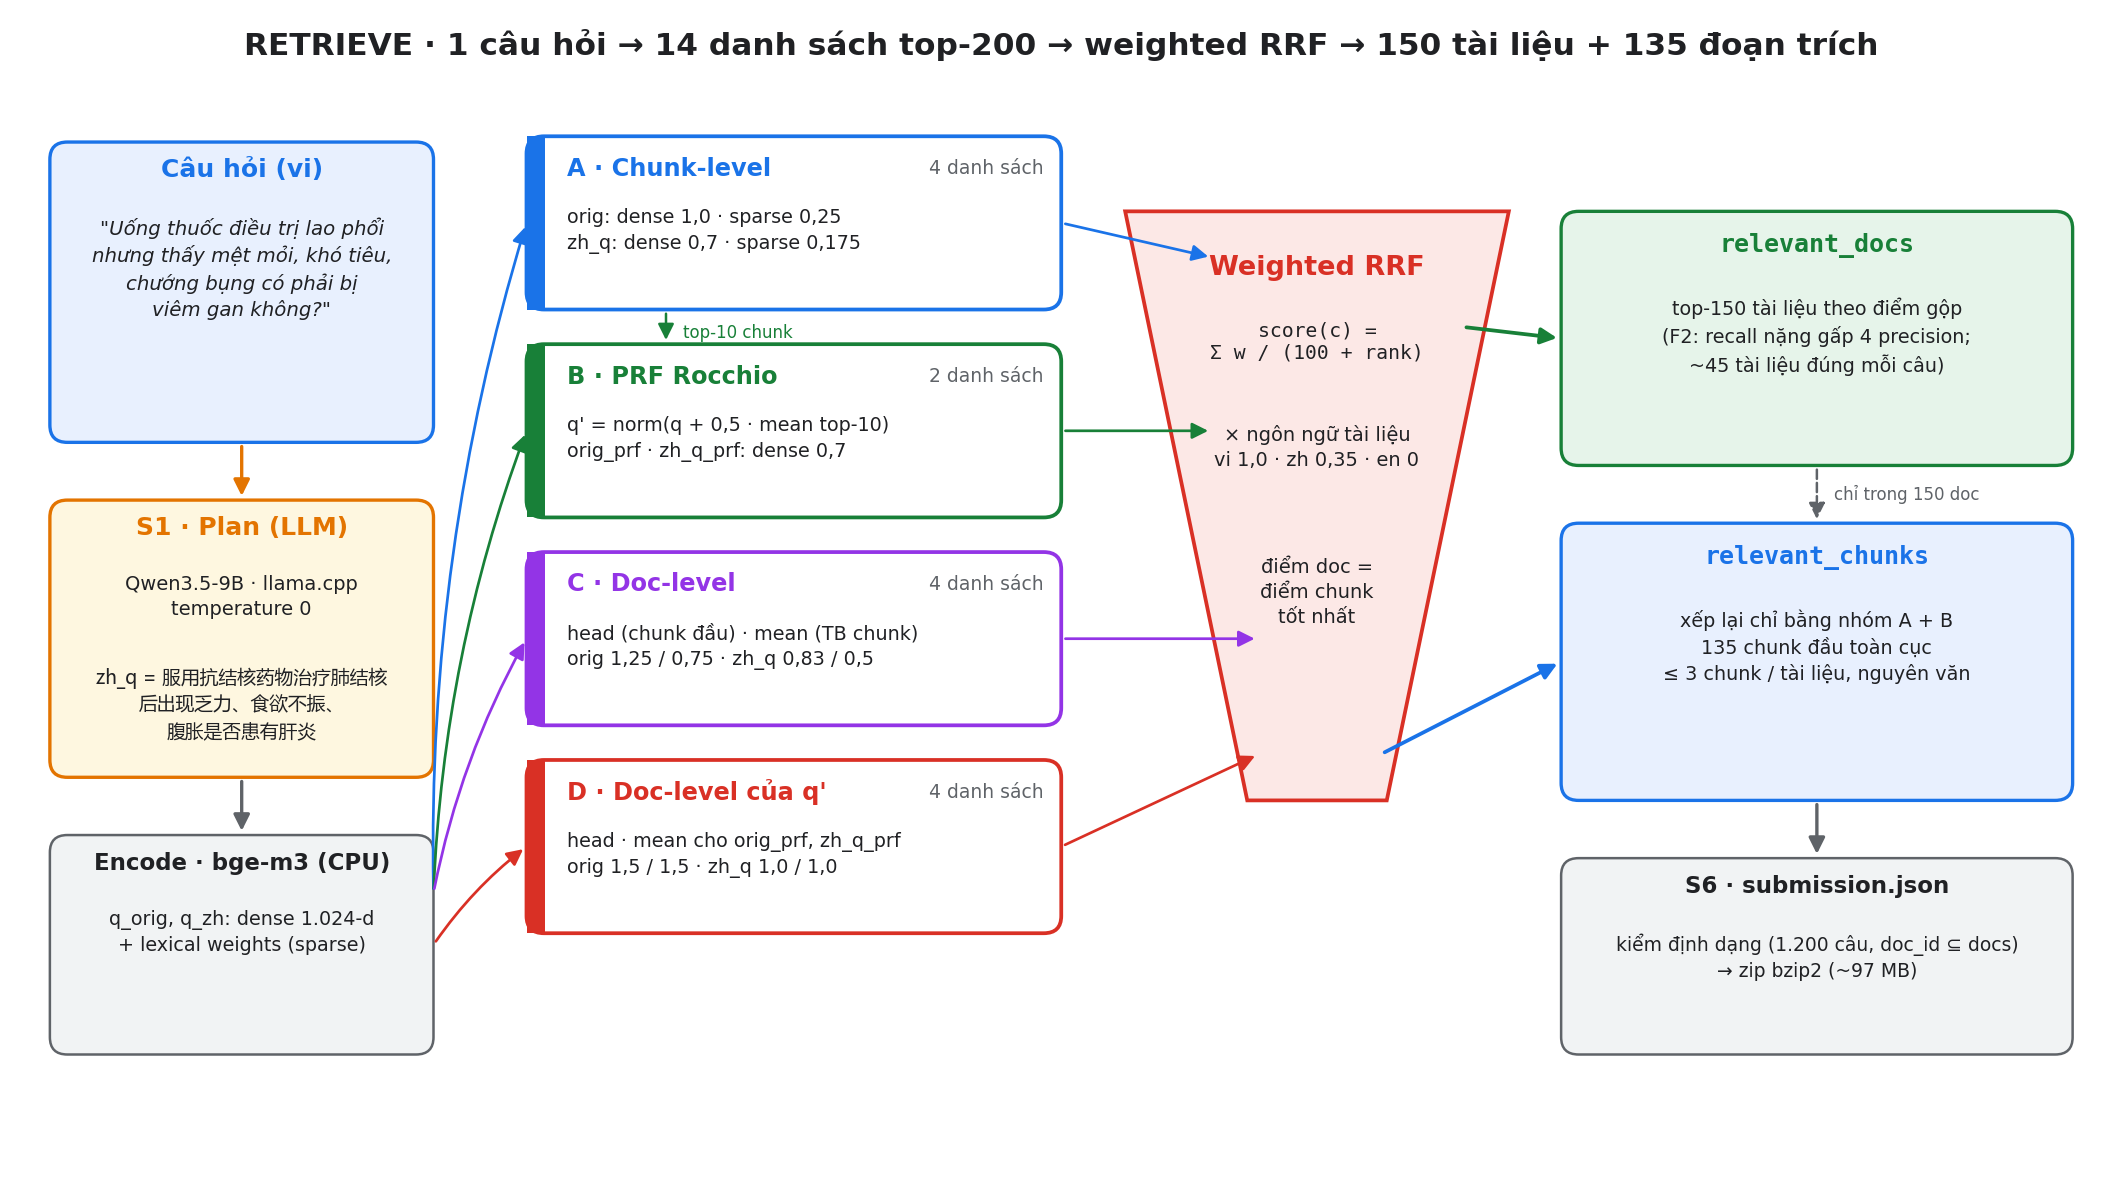
\includegraphics[width=\linewidth]{../img/retrieve.png}\\[2pt]
{\small\color{mute}Hình 2. Pha retrieve: 14 danh sách thuộc 4 nhóm, gộp bằng weighted RRF.}
\end{center}

\begin{enumerate}[label={\color{brand}\headfont\arabic*.},leftmargin=1.6em,itemsep=5pt]
\item \textbf{Plan.} Qwen3.5-9B dịch câu hỏi sang tiếng Trung theo kiểu tiêu đề diễn đàn (\texttt{zh\_q}), để khớp các trang hỏi đáp như 120ask hay 39.net.
\item \textbf{Encode.} Câu gốc và bản dịch được mã hoá bằng BGE-M3 thành vector dense và trọng số sparse.
\item \textbf{Bốn nhóm danh sách,} mỗi danh sách lấy top-200:
  \begin{itemize}
  \item \textbf{A · Cấp chunk.} Dense trên chỉ mục vi + zh, sparse trên chỉ mục cùng ngôn ngữ; cho cả câu gốc và \texttt{zh\_q}.
  \item \textbf{B · Rocchio PRF.} Tạm coi 10 chunk đầu là đúng, kéo câu hỏi về phía chúng rồi tìm lại:
  $q' = \mathrm{norm}\big(q + 0{,}5\cdot\overline{v}_{\text{top-10}}\big)$.
  Câu hỏi đời thường nhờ vậy có thêm thuật ngữ chuyên môn.
  \item \textbf{C · Cấp tài liệu.} So câu hỏi trực tiếp với vector head và mean của từng tài liệu. Nhóm này ưu tiên tài liệu mà \emph{cả bài} nói về chủ đề, không chỉ một đoạn.
  \item \textbf{D · Cấp tài liệu của $q'$.} Như nhóm C, nhưng dùng câu hỏi đã mở rộng.
  \end{itemize}
\item \textbf{Weighted RRF.} Mỗi chunk được cộng điểm từ mọi danh sách có chứa nó, rồi nhân với trọng số ngôn ngữ của tài liệu:
  \[ \mathrm{score}(c) = \lambda_{\mathrm{lang}(c)} \sum_{\ell} \frac{w_\ell}{100 + \mathrm{rank}_\ell(c)} \]
  Điểm tài liệu là điểm chunk tốt nhất của nó.
\item \textbf{Chọn đầu ra.} \texttt{relevant\_docs} là 150 tài liệu đầu. \texttt{relevant\_chunks} được xếp lại chỉ bằng nhóm A + B (tín hiệu cấp đoạn): lấy 135 chunk đầu toàn cục thuộc 150 tài liệu đó, tối đa 3 chunk mỗi tài liệu. Mỗi đoạn trích là nguyên văn một chunk.
\end{enumerate}

\begin{note}[colback=ambersoft,colframe=ambersoft,borderline west={3pt}{0pt}{amber}]
\textbf{Vì sao chọn các con số này?} Mỗi câu hỏi có khoảng 45 tài liệu đúng và F2 thưởng recall, nên nộp 150 tài liệu. Gold không chứa PubMed nên tiếng Anh nhân 0; gold có ít tài liệu tiếng Trung nên tiếng Trung nhân 0,35. Mọi trọng số đều được chọn qua các lần nộp vòng public, mỗi lần đổi một yếu tố. Reranker cross-encoder, LLM judge, HyDE và mô hình nhúng thứ hai (e5) đều đã được thử và bị loại vì không cải thiện điểm.
\end{note}

\begin{codebox}{Cấu hình bài nộp i\_dprf15 · configs/deep\_bge\_vizh\_k100.json + bench/variants.py}
\begin{Verbatim}
# truy hồi
dense_langs = sparse_langs = ["vi", "zh"];  k_dense = k_sparse = 200
prf = {"n": 10, "alpha": 0.5};  doc_level_k = 200
# gộp
rrf_k = 100;  w_dense, w_sparse = 1.0, 0.25;  w_trans = 0.7      # zh_q, orig_prf, zh_q_prf
variant_weight = {"orig_head": 1.25, "zh_q_head": 0.833, "orig_mean": 0.75, "zh_q_mean": 0.5,
                  "orig_prf_head": 1.5, "zh_q_prf_head": 1.0, "orig_prf_mean": 1.5, "zh_q_prf_mean": 1.0}
lang_weight = {"vi": 1.0, "zh": 0.35, "en": 0.0}
# chọn
k_docs = 150;  chunk_lists = ["orig", "zh_q", "orig_prf", "zh_q_prf"]
chunk_global = 135;  k_chunks_per_doc = 3
\end{Verbatim}
\end{codebox}

\vspace{6pt}{\headfont\large\color{brand}Ví dụ: câu hỏi số 13}\par\vspace{2pt}
\begin{tcolorbox}[enhanced,colback=white,colframe=line,boxrule=0.6pt,arc=3pt,left=10pt]
\itshape "Uống thuốc điều trị lao phổi nhưng thấy người mệt mỏi, ăn uống khó tiêu, chướng bụng có phải bị viêm gan không?"
\end{tcolorbox}

\textbf{Bước 1 · Plan.} Qwen3.5-9B trả về \texttt{zh\_q = }服用抗结核药物治疗肺结核后出现乏力、食欲不振、腹胀是否患有肝炎, kèm thực thể \emph{thuốc điều trị lao phổi} → \emph{anti-tuberculosis medication} → 抗结核药物.

\textbf{Bước 2–3 · Các danh sách.} Ba kết quả đầu của một số danh sách:

\begin{nicetable}{@{}p{3.4cm}p{1.2cm}Y@{}}
\thead{Danh sách} & \thead{Nhóm} & \thead{Top-3 (doc:chunk)} \\ \midrule
\texttt{orig} dense & A & 277870:0 · 554196:0 · \textbf{568969:0} \\
\texttt{orig} sparse & A & 277870:0 · 135240:1 · 568969:1 \\
\texttt{zh\_q} dense & A & 2390048:0 · 2370138:0 · 2941973:0 \\
\texttt{orig\_prf} dense & B & \textbf{568969:0} · 554196:0 · 277870:0 \\
\texttt{orig\_mean} & C & \textbf{568969:0} · 277870:0 · 522515:0 \\
\texttt{orig\_prf\_mean} & D & \textbf{568969:0} · 522515:0 · 275481:0 \\
\bottomrule
\end{nicetable}

PRF và các danh sách cấp tài liệu cùng đẩy bài chuyên đề 568969 lên đầu, trong khi danh sách dense của câu gốc chỉ xếp bài này thứ 3.

\textbf{Bước 4–5 · Kết quả nộp:} 150 tài liệu (143 tiếng Việt, 7 tiếng Trung) và 135 đoạn trích.

\begin{nicetable}{@{}>{\raggedleft\arraybackslash}p{1.1cm}p{1.8cm}Y@{}}
\thead{Hạng} & \thead{doc\_id} & \thead{Tiêu đề} \\ \midrule
1 & 568969 & VIÊM GAN DO SỬ DỤNG THUỐC KHÁNG LAO \\
2 & 277870 & Uống thuốc lao bị mệt có nguy hiểm không? \\
3 & 554196 & Tổn thương gan do dùng isoniazid \\
4 & 551684 & Thuốc chống lao có thể gây độc cho gan \\
5 & 509817 & Đang điều trị lao có nên uống thuốc bổ gan? \\
135 & 2390048 & 肺结核药物性肝炎症状是什么 {\color{mute}\small(triệu chứng viêm gan do thuốc lao)} \\
138 & 2370138 & 抗结核药物造成肝损害的症状 {\color{mute}\small(tổn thương gan do thuốc chống lao)} \\
\bottomrule
\end{nicetable}

Các tài liệu tiếng Trung chỉ có mặt nhờ bản dịch \texttt{zh\_q}, và đứng cuối danh sách vì bị nhân trọng số 0,35.

% ================================================================= 4
\section{Tham khảo}

\begin{tcolorbox}[enhanced,colback=brandsoft,colframe=brandsoft,arc=4pt,halign=center,top=10pt,bottom=10pt]
{\headfont Mã nguồn, dữ liệu, checkpoint và hướng dẫn cài đặt, chạy lại}\\[4pt]
\href{https://github.com/quaqducc/r2ai-stage3-medical-retrieval}{\color{brand}\large https://github.com/quaqducc/r2ai-stage3-medical-retrieval}\\[2pt]
{\small\color{mute}(xem README.md)}
\end{tcolorbox}

\end{document}
